\documentclass[a4paper,14pt]{extarticle}

\def\labauthors{Сарафанов Ф.Г., Платонова М.В.}
\def\labgroup{440}
\def\labnumber{1}
\def\labstartdate{3 декабря}
\def\labtheme{Оценивание параметров  \\[0.2em] случайного процесса}
\def\shortlabtheme{Параметры случайного процесса}

%!TEX root = ../fet.tex
\usepackage{cmap}
\usepackage[T2A]{fontenc}
\usepackage[utf8x]{inputenc}
\usepackage[english, russian]{babel}

\usepackage{misccorr} % в заголовках появляется точка, но при ссылке на них ее нет
\usepackage{amssymb,amsfonts,amsmath,amsthm}  
\usepackage{indentfirst}
\usepackage[usenames,dvipsnames]{color} 
\usepackage[unicode,hidelinks]{hyperref}
% \hypersetup{%
%     pdfborder = {0 0 0}
% }

\usepackage{makecell,multirow} 
\usepackage{ulem}
\usepackage{graphicx,wrapfig}
\graphicspath{{img/}}
\usepackage{geometry}
\geometry{left=2cm,right=2cm,top=3cm,bottom=3cm,bindingoffset=0cm,headheight=15pt}
\usepackage{fancyhdr} 
\linespread{1.05} 
\frenchspacing 
\renewcommand{\labelenumii}{\theenumii)} 
\newcommand{\mean}[1]{\langle#1\rangle}
% \usepackage{caption}
%%%%%%%%%%%%%%%%%%%%%%%%%%%%%%%%%%%%%%%%%%%%%%%%%%%%%%%%%%%%%%%%%%%%%%%%%%%%%%%
%%%%%%%%%%%%%%%%%%%%%%%%%%%%%%%%%%%%%%%%%%%%%%%%%%%%%%%%%%%%%%%%%%%%%%%%%%%%%%%



%%%%%%%%%%%%%%%%%%%%%%%%%%%%%%%%%%%%%%%%%%%%%%%%%%%%%%%%%%%%%%%%%%%%%%%%%%%%%%%
	%применим колонтитул к стилю страницы
\pagestyle{fancy} 
	%очистим "шапку" страницы
\fancyhead{} 
	%слева сверху на четных и справа на нечетных
\fancyhead[L]{\labauthors} 
	%справа сверху на четных и слева на нечетных
\fancyhead[R]{\shortlabtheme} 
	%очистим "подвал" страницы
\fancyfoot{} 
	% номер страницы в нижнем колинтуле в центре
\fancyfoot[C]{\thepage} 
\renewcommand{\phi}{\varphi}
%%%%%%%%%%%%%%%%%%%%%%%%%%%%%%%%%%%%%%%%%%%%%%%%%%%%%%%%%%%%%%%%%%%%%%%%%%%%%%%

\usepackage{float}
\usepackage[mode=buildnew]{standalone}
\usepackage{tikz} 
% \usepackage{subcaption}
\usepackage{csvsimple}
\usetikzlibrary{scopes}
\usetikzlibrary{%
     decorations.pathreplacing,%
     decorations.pathmorphing,%
    patterns,%
    calc,%
    scopes,%
    arrows,%
    % arrows.spaced,%
}
\makeatletter
\newif\if@gather@prefix 
\preto\place@tag@gather{% 
  \if@gather@prefix\iftagsleft@ 
    \kern-\gdisplaywidth@ 
    \rlap{\gather@prefix}% 
    \kern\gdisplaywidth@ 
  \fi\fi 
} 
\appto\place@tag@gather{% 
  \if@gather@prefix\iftagsleft@\else 
    \kern-\displaywidth 
    \rlap{\gather@prefix}% 
    \kern\displaywidth 
  \fi\fi 
  \global\@gather@prefixfalse 
} 
\preto\place@tag{% 
  \if@gather@prefix\iftagsleft@ 
    \kern-\gdisplaywidth@ 
    \rlap{\gather@prefix}% 
    \kern\displaywidth@ 
  \fi\fi 
} 
\appto\place@tag{% 
  \if@gather@prefix\iftagsleft@\else 
    \kern-\displaywidth 
    \rlap{\gather@prefix}% 
    \kern\displaywidth 
  \fi\fi 
  \global\@gather@prefixfalse 
} 
\newcommand*{\beforetext}[1]{% 
  \ifmeasuring@\else
  \gdef\gather@prefix{#1}% 
  \global\@gather@prefixtrue 
  \fi
} 
\makeatother

\usepackage{booktabs}
\usepackage{pgfplots, pgfplotstable}

\usepackage[outline]{contour}
\usepackage{tocloft}
\renewcommand{\cftsecleader}{\cftdotfill{\cftdotsep}} % for parts
% \renewcommand{\cftchapleader}{\cftdotfill{\cftdotsep}} % for chapters
\usepackage{pgfplots,pgfplotstable,booktabs,colortbl}
\pgfplotsset{compat=newest}
\usepackage{physics}
\usepackage{mathtools}
\mathtoolsset{showonlyrefs=true}
\newcommand\Smat{\hat { \mathbf { S } }}

\newcommand*\dotvec[1][1,1]{\crossproducttemp#1\relax}
\def\crossproducttemp#1,#2\relax{{\qty[\vec{#1}\times\vec{#2}\,]}}

\newcommand*\prodvec[1][1,1]{\crossproducttempa#1\relax}
\def\crossproducttempa#1,#2\relax{{\qty[{#1}\times{#2}\,]}}

% \def\E{\mathscr{E}_H}
\def\Rdim{\,\frac{\text{м}^3}{\text{А} \cdot \text{с}}}

\renewcommand{\vec}{\mathbf} % for parts
\newcommand{\D}[1]{D\qty[#1]}

\begin{document}
%!TEX root = ../fet.tex
\begin{titlepage}
\begin{center}
% \vspace{-3em}
{\small\textsc{Нижегородский государственный университет имени Н.\,И. Лобачевского}}
\vskip 2pt \hrule \vskip 3pt
{\small\textsc{Радиофизический факультет}}

\vfill


{{\large Отчет по лабораторной работе №\labnumber}\vskip 12pt {\LARGE \bfseries \labtheme}}

	
\vspace{2cm}
{\large Работу выполнили студенты \\[-0.25em] \labgroup\  группы радиофизического факультата \\[0.5em] {\Large \bfseries \labauthors}}

% \vspace{0.5cm}
% {e-mail: sfg180@yandex.ru}

% \vspace{2cm}

\end{center}

\vfill
	
% \begin{flushright}
% 	{Выполнили студенты 430 группы\\ \labauthor}%\vskip 12pt Принял:\\ Менсов С.\,Н.}
% \end{flushright}
	
% \vfill
	
\begin{center}
	{Нижний Новгород, \labstartdate\ -- \today}
\end{center}

\end{titlepage}

\tableofcontents
\newpage



\addcontentsline{toc}{section}{Введение}
\section*{Введение}
% \vspace{-0.5em}
В настоящей работе изучаются вопросы, связанные с оценкой параметров случайных процессов, на примере оценки среднего значения (матожидания) случайного процесса.

\paragraph{Краткие теоретические материалы.} В работе используется ряд понятий и формул. Не вдаваясь в конспектирование методических материалов\footnotemark, приведем лишь основные формулы, полезные для понимания работы. \\[0.5em]
\textit{Оценка среднего значения случайного процесса}
\begin{equation}
     \tilde x = \frac{1}{n} \sum\limits_{i=1}^{n} x_i(t_i) 
 \end{equation} 
\textit{Среднеквадратичное отклонение и дисперсия эргодического процесса}
\begin{equation}
    \mathrm{D}\qty[\tilde x] = \frac{\mathrm{D}\qty[x]}{n} + \frac{1}{n^2} \sum\limits_{i=1}^{n} \sum\limits_{j\neq i}^{n} \mathrm{B}_x(t_i - t_j), \quad \sigma_{\tilde x} = \sqrt{\mathrm{D}\qty[\tilde x]}
\end{equation}
\textit{Определение дисперсии из СПМ}
\begin{equation}
    \mathrm{D}[\tilde x]=S_{\tilde x}(0)\cdot \Delta f_{\tilde x} = S_{\tilde x}(0) \frac{1}{2T}
\end{equation}
\textit{Связь доверительной вероятности и доверительного интервала с $W(\tilde x)$}
\begin{equation}
    P\qty(\abs{\mean{x}} - \tilde x \leq I_{\beta}) = \int\limits_{\mean{x}-I_{\beta}}^{\mean{x}+I_{\beta}}  W(\tilde x) \dd{\tilde x} = \beta
\end{equation}


\footnotetext{Артюхин И.В., Болховская О.В. и другие. Лабораторные работы по курсу <<статистическая радиофизика>>. Практикум. -- Н.Новгород:ННГУ, 2010. -- 78 c.}



\newpage


\section{Лабораторный эксперимент}
Для выполнения лабораторной работы использовалась вспомогательная программа, предоставляющая возможность сгенерировать гауссов шум с заданным временем корреляции $\tau_\text{корр}$, усреднить $M$ реализаций скользящим средним с регулируемыми шириной окна $N$, периодом дискретизации $\Delta t$.

Для сгенерированного сигнала программа позволяет рассчитать среднее значение, СКО и доверительный интервал, получить графики зависимостей СКО от параметров усреднения, графики реализаций и спектров, гистограммы оценок среднего значения.

\subsection{Реализации случайных процессов и их спектров}

Для иллюстрации случайных процессов были сгенерированы реализации дискретного гауссова шума для разных времен корреляции $\tau_\text{корр}$ (10,30,100) и построены графики как самих реализаций, так и их СПМ\footnote{СПМ -- здесь и далее -- спектральная плотность мощности}.

\begin{figure}[H]
    \centering
    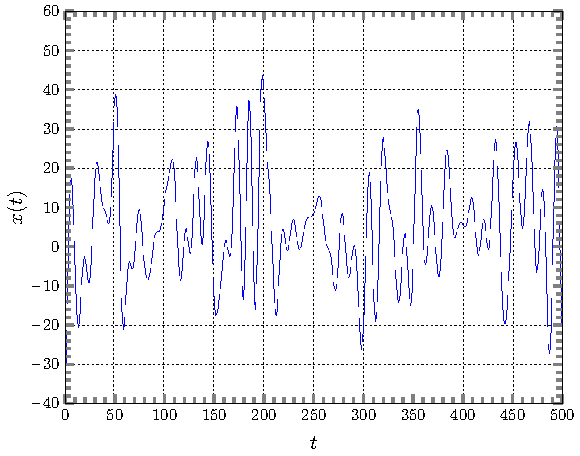
\includegraphics[width=0.7\linewidth]{fig/x_from_t_10.pdf}
    \vspace{-0.7em}
    \caption{Реализация случайного процесса с $\tau_\text{корр}=10$}
    \label{fig:t10}
\end{figure}

\begin{figure}[H]
    \centering
    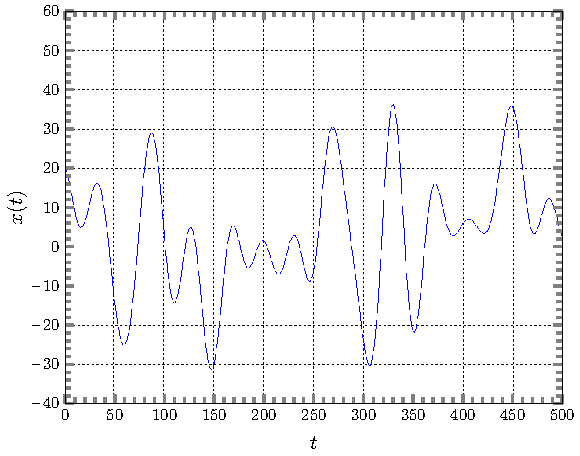
\includegraphics[width=0.7\linewidth]{fig/x_from_t_30.pdf}
    \vspace{-0.7em}
    \caption{Реализация случайного процесса с $\tau_\text{корр}=30$}
    \label{fig:t30}
\end{figure}


\begin{figure}[H]
    \centering
    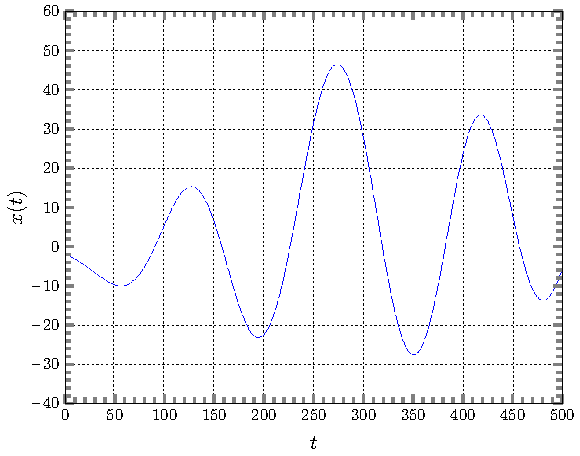
\includegraphics[width=0.7\linewidth]{fig/x_from_t_100.pdf}
    \vspace{-0.7em}
    \caption{Реализация случайного процесса с $\tau_\text{корр}=100$}
    \label{fig:t100}
\end{figure}

\begin{figure}[H]
    \centering
    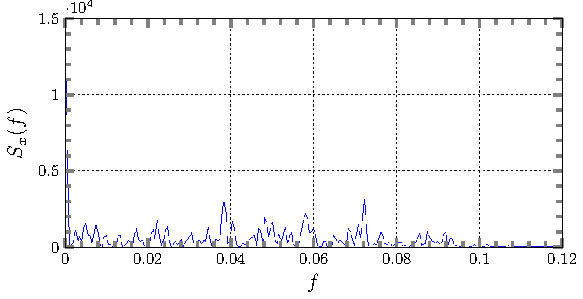
\includegraphics[width=0.7\linewidth]{fig/S_from_f_10.pdf}
    \vspace{-0.7em}
    \caption{СПМ случайного процесса с $\tau_\text{корр}=10$}
    \label{fig:s10}
\end{figure}

\begin{figure}[H]
    \centering
    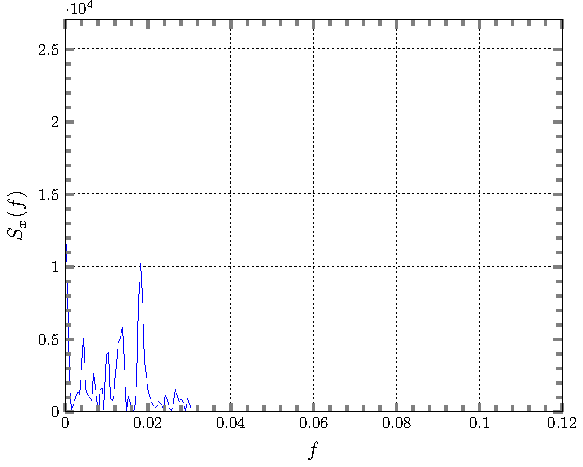
\includegraphics[width=0.7\linewidth]{fig/S_from_f_30.pdf}
    \vspace{-0.7em}
    \caption{СПМ случайного процесса с $\tau_\text{корр}=30$}
    \label{fig:s30}
\end{figure}

\begin{figure}[H]
    \centering
    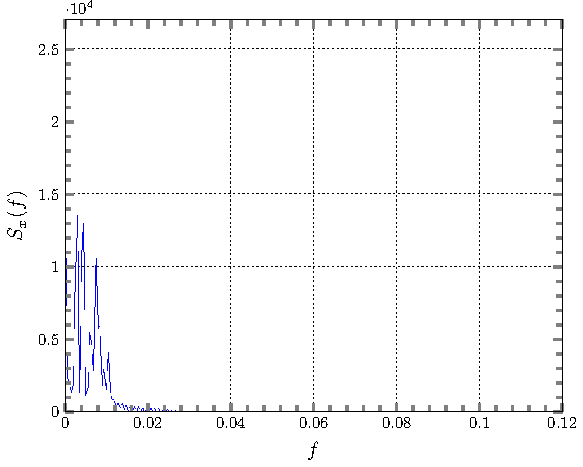
\includegraphics[width=0.7\linewidth]{fig/S_from_f_100.pdf}
    \vspace{-0.7em}
    \caption{СПМ случайного процесса с $\tau_\text{корр}=100$}
    \label{fig:s100}
\end{figure}

На графиках СПМ (см. рис. \ref{fig:s10}, \ref{fig:s30}, \ref{fig:s100}) хорошо видно, что ширина спектра обратно пропорциональна времени корреляции\footnote{Время корреляции $\tau_\text{кор}$  -- это время, при котором функция корреляции $\mathrm{B}[\tau]$ спадает в $e$ раз}. Это объясняется тем, что при больших временах корреляции два близких во времени отсчета сигнала отличаются слабо и сигнал меняется медленно, следовательно, имеет меньшую ширину спектра. Для малых времен применимы аналогичные рассуждения.


\subsection{Зависимость $\mean{x}$ от ширины окна усреднения $N$}
При заданных времени корреляции генерируемого сигнала $t_\text{корр}=10$, числе реализаций $M=128$, времени дискретизации $\Delta t=1$, ширине окна усреднения (количество усредняемых отсчетов) $N=1$ с помощью программы определены оценки среднего и СКО:
\begin{equation}
    \mean{x}=4.68, \quad \sigma_x = 14.74
\end{equation}

Также при времени корреляции генерируемого сигнала $t_\text{корр}=10$, числе реализаций $M=8$, времени дискретизации $\Delta t=1$ определена зависимость оценки от ширины окна усреднения ($N$):
\begin{figure}[H]
    \centering
    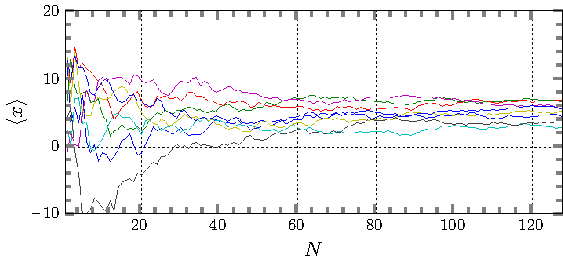
\includegraphics[width=0.8\textwidth]{fig/mean_from_N}
    \caption{Оценка среднего в зависимости от числа усредняемых отсчетов}
    \label{fig:mean_from_n}
\end{figure}

Разброс среднего от вертикали определяет собой \textit{дисперсию}. Разброс при $N=1$ составляет $\delta \mean{x}\approx15$, при $N=40$ соответственно $\delta \mean{x}\approx8$, и при $N=128$, наконец, $\delta \mean{x}\approx5$.





\subsection{Зависимость $\sigma_x$ от ширины окна усреднения $N$}
При заданных времени корреляции генерируемого сигнала $t_\text{корр}=10$, числе реализаций $M=256$, найдена серия зависимостей зависимость оценки от ширины окна усреднения ($N$) при разных временах дискретизации:
\begin{figure}[H]
    \centering
    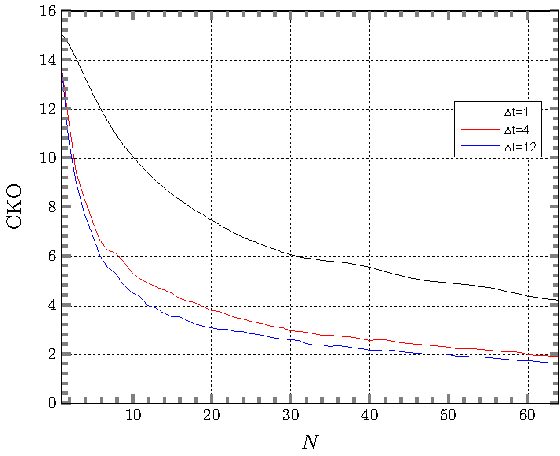
\includegraphics[width=0.8\textwidth]{fig/sko_t10.pdf}
    \caption{Зависимость СКО от числа усредняемых отсчетов}
    \label{fig:sko_from_n_t10}
\end{figure}
На графике видно, что с ростом времени корреляции СКО уменьшается. Действительно, так как оценка среднего совпадет\footnotemark{} с истинным значением при $T \to \infty$, то увеличивая время корреляции, мы приближаемся к условию $T \to \infty$, а значит, уменьшаем СКО.
\footnotetext{
Оценка среднего случайного процесса определяется как
\begin{equation}
    \label{eq:}
    \tilde x(t) = \lim_{T \to \infty} \int\limits_{0}^{T = n\cdot \tau_{\text{кор}}}  x(t) \dd{t}
\end{equation}}



\newpage
Аналогичная серия при тех же параметрах, но времени корреляции 100:
\begin{figure}[H]
    \centering
    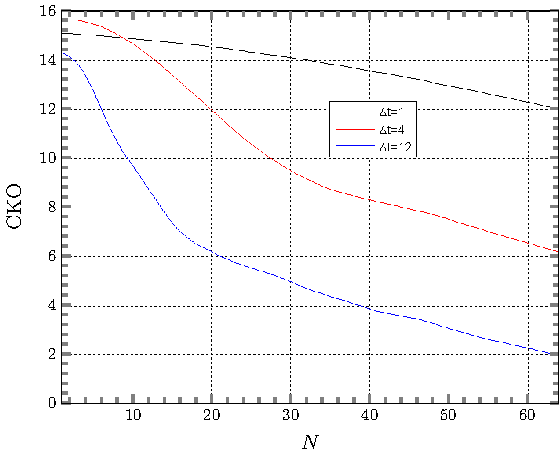
\includegraphics[width=0.8\textwidth]{fig/sko_t100.pdf}
    \caption{Зависимость СКО от числа усредняемых отсчетов}
    \label{fig:sko_from_n_t100}
\end{figure}
Заметим, что можно оценить время корреляции процесса по графику. Так как в случае $\Delta t \cdot N^* \ge \tau_\text{кор}$ 
\begin{equation}
    D[\tilde{x}] = \frac{D[x]}{N},
\end{equation}
то график $\sigma_x(N)$ после $\Delta t \cdot N^* = \tau_\text{кор}$ будет вести себя как гипербола. По точке перехода графика в гиперболу $N^*$ можно определить $\tau_\text{кор}$.

СКО оценки при $N=1$ определяется числом реализаций сигнала $M$. В таком случае для каждой реализации среднее значение - это значение единственного элемента в реализации. Другими словами, СКО оценки при $N=1$ определяется как дисперсия исходного процесса $D[x]$.



\subsection{Зависимость $\sigma_x$ от времени дискретизации $\Delta t$}

\begin{figure}[H]
    \centering
    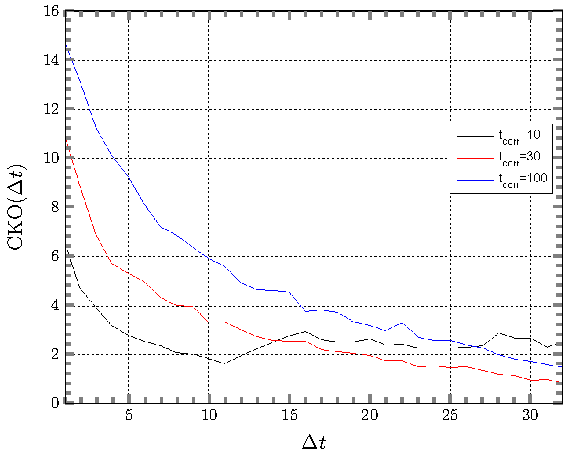
\includegraphics[width=0.7\linewidth]{fig/sko_n4.pdf}
    \vspace{-0.7em}
    \caption{$N=4$}
    \label{fig:sko_n4}
\end{figure}

\begin{figure}[H]
    \centering
    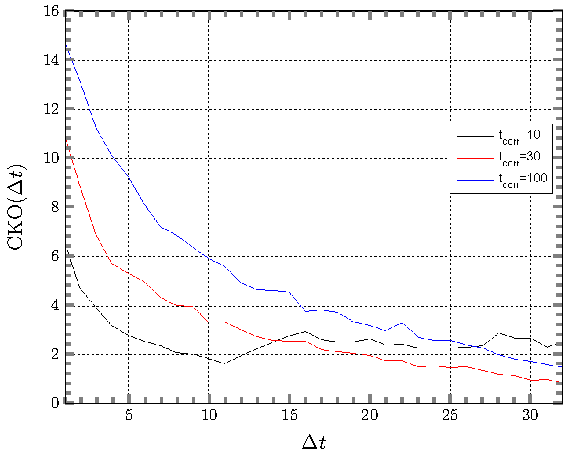
\includegraphics[width=0.7\linewidth]{fig/sko_n32.pdf}
    \vspace{-0.7em}
    \caption{$N=32$}
    \label{fig:sko_n32}
\end{figure}




\subsection{Определение $\mean{x}$ и $\sigma_x$ по  СПМ процесса}

\subsubsection{Параметры исходного процесса}

\begin{figure}[H]
    \centering
    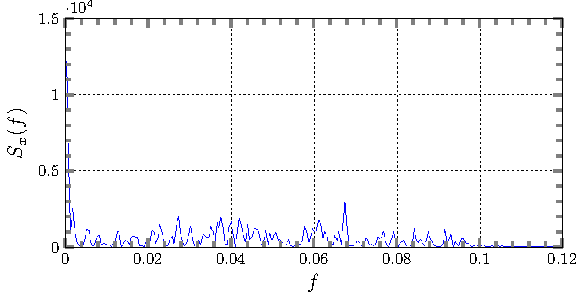
\includegraphics[width=0.7\linewidth]{fig/S_from_f_100_ex51}
    \vspace{-0.7em}
    \caption{$N=32$}
    \label{fig:sko_ex51}
\end{figure}

С помощью лабораторной программы строится график СПМ при $N=32$, $\tau_\text{корр}=10$. Из графика находится значение СПМ в нуле
\begin{equation}
    S_x(0) = 1.2\cdot 10^4
\end{equation}
Так как полная мощность в полосе $\Delta\omega = \frac{1}{2048}$ на нулевой частоте равна (с некоторой погрешностью) $\mean{x}^2 = S_x(0)\cdot \frac{1}{2048}$, то
\begin{equation}
    \mean{x}^2 = 1.2\cdot 10^4\cdot \frac{1}{2048} = 5.86
    \quad \Rightarrow \quad \mean{x}=2.42
\end{equation}
Из графика СПМ также можно найти дисперсию как произведение эффективной ширины спектра на эффективное значение СПМ:
\begin{equation}
    \mathrm{D}[\tilde{x}] = S_x(0)\cdot \Delta f_{\tilde{x}} =\frac{\mean{x}^2}{2} = 2.93 
    \quad \Rightarrow \quad
    \sigma_{\tilde{x}} = \sqrt{D[\tilde{x}]}\approx 1.71
\end{equation}


\subsubsection{Параметры усредненного процесса}

\begin{figure}[H]
    \centering
    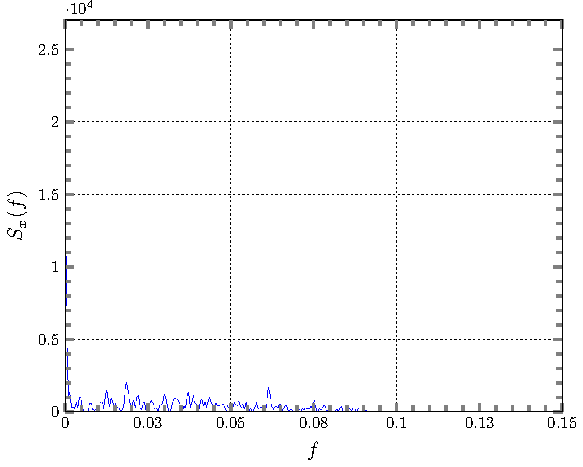
\includegraphics[width=0.7\linewidth]{fig/S_from_f_100_ex52_n4}
    \vspace{-0.7em}
    \caption{$N=4$}
    \label{fig:sko_ex52_n4}
\end{figure}

Аналогично операциям с исходным процессом, из графика при ширине окна усреднения $N=4$ находится величина СПМ в нуле, и простым расчетом находится среднее и дисперсия:
\begin{equation}
    S_x(0) = 1.25 \cdot 10^4
    \quad \Rightarrow \quad
    \mean{x}=2.43, \quad
    \sigma_{\tilde{x}} =  1.72
\end{equation}


\begin{figure}[H]
    \centering
    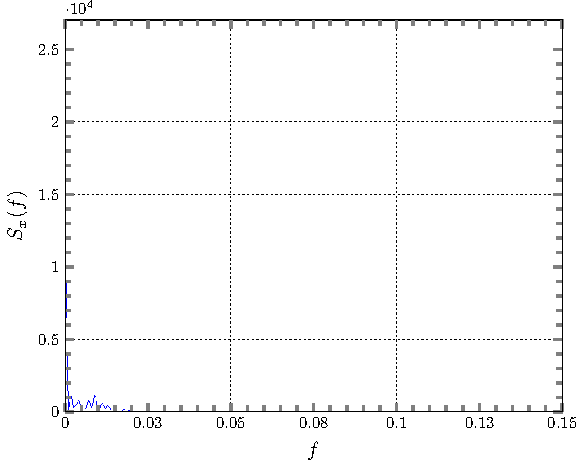
\includegraphics[width=0.7\linewidth]{fig/S_from_f_100_ex52_n32}
    \vspace{-0.7em}
    \caption{$N=32$}
    \label{fig:sko_ex52_n32}
\end{figure}

При усреднении с шириной окна $N=32$ получаются следующие параметры:
\begin{equation}
    S_x(0) = 1 \cdot 10^4
    \quad \Rightarrow \quad
    \mean{x}=1.99, \quad
    \sigma_{\tilde{x}} =  1.41
\end{equation}

\subsection{Доверительный интервал}
Можно исследовать влияние времени усреднения и доверительной вероятности на доверительный интервал. Для этого с помощью лабораторной программы построены гистограммы, иллюстрирующие распределение значений ансамбля из $M=256$ оценок среднего.

\subsubsection{Анализ гистограммы}
При заданных времени корреляции $\tau = 10$ и доверительной вероятности $\beta=0.95$, времени дискретизации $\Delta t=1$ получена серия гистограмм при разных ширинах окна усреднения $N=1, 4, 32$, отображенная на рисунках \ref{fig:g1}, \ref{fig:g4}, \ref{fig:g32}:
\vfill
\begin{figure}[H]
    \centering
    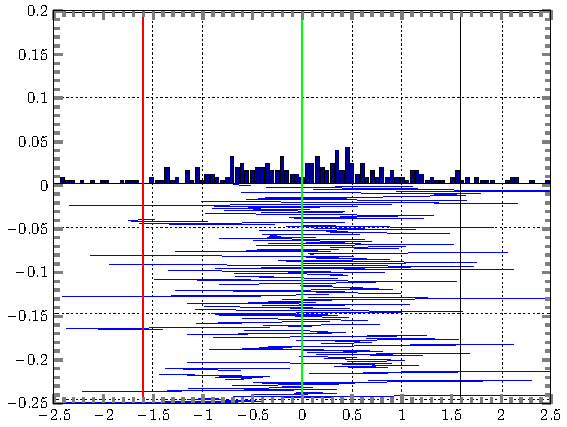
\includegraphics[width=0.75\linewidth]{fig/gist_n1}
    \vspace{-0.7em}
    \caption{$N=1$}
    \label{fig:g1}
\end{figure}
\vfill
\newpage
\begin{figure}[H]
    \centering
    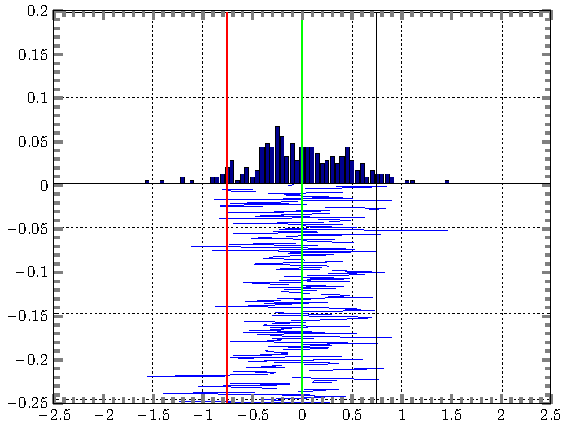
\includegraphics[width=0.75\linewidth]{fig/gist_n4}
    \vspace{-0.7em}
    \caption{$N=4$}
    \label{fig:g4}
\end{figure}
\begin{figure}[H]
    \centering
    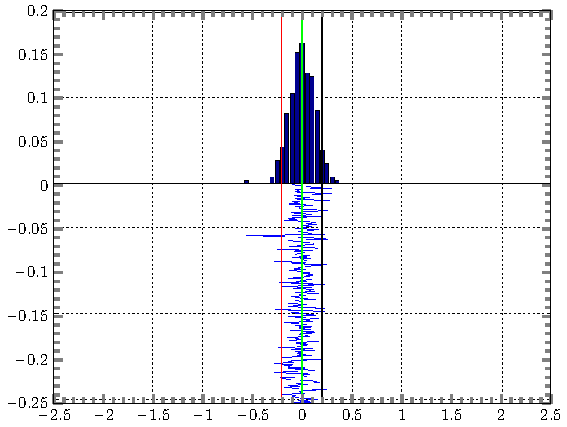
\includegraphics[width=0.75\linewidth]{fig/gist_n32}
    \vspace{-0.7em}
    \caption{$N=32$}
    \label{fig:g32}
\end{figure}
\subsubsection{Влияние доверительной вероятности}
При заданных времени корреляции $\tau = 10$, времени дискретизации $\Delta t=1$ получена серия $3\times3$ гистограмм при разных ширинах окна усреднения $N=1, 4, 32$ и разных доверительных вероятностях $\beta=0.8, 0.95, 0.98$:

\paragraph{Серия при $N=1$.} \hphantom{asasfsd}
\begin{figure}[H]
\begin{minipage}{0.3\linewidth}
    \centering
    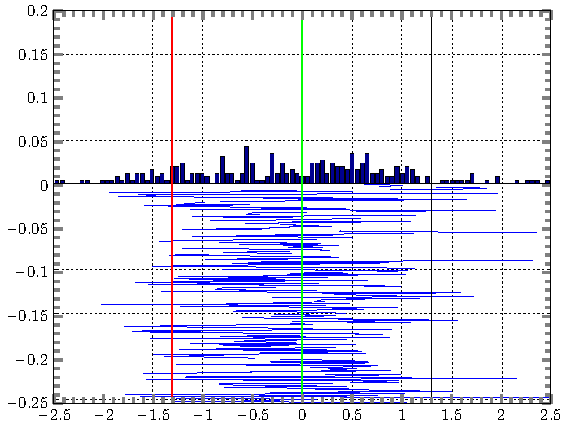
\includegraphics[width=\linewidth]{fig/gist_n1_b80.pdf}
    \vspace{-1em}
    \caption{$\beta =0.8$}
\end{minipage}
\begin{minipage}{0.3\linewidth}
    \centering
    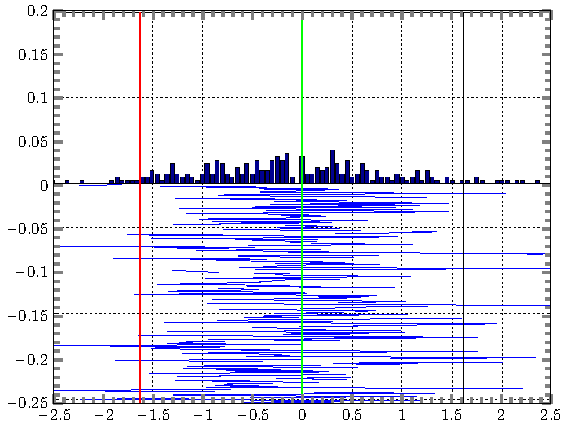
\includegraphics[width=\linewidth]{fig/gist_n1_b95.pdf}
    \vspace{-1em}
    \caption{$\beta =0.95$}
\end{minipage}
\begin{minipage}{0.3\linewidth}
    \centering
    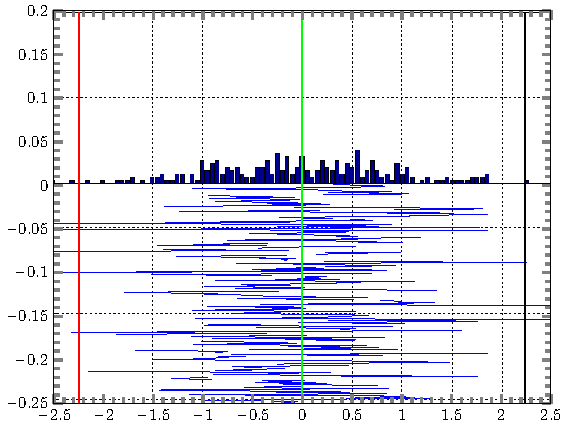
\includegraphics[width=\linewidth]{fig/gist_n1_b98.pdf}
    \vspace{-1em}
    \caption{$\beta =0.98$}
\end{minipage}
\end{figure}

\paragraph{Серия при $N=4$.} \hphantom{asasfsd}
\begin{figure}[H]
\begin{minipage}{0.3\linewidth}
    \centering
    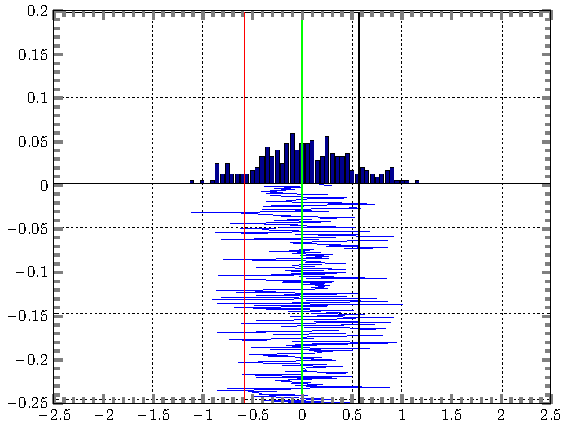
\includegraphics[width=\linewidth]{fig/gist_n4_b80.pdf}
    \vspace{-1em}
    \caption{$\beta =0.8$}
\end{minipage}
\begin{minipage}{0.3\linewidth}
    \centering
    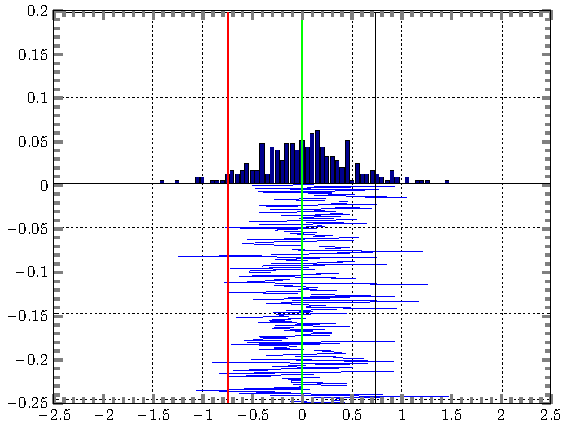
\includegraphics[width=\linewidth]{fig/gist_n4_b95.pdf}
    \vspace{-1em}
    \caption{$\beta =0.95$}
\end{minipage}
\begin{minipage}{0.3\linewidth}
    \centering
    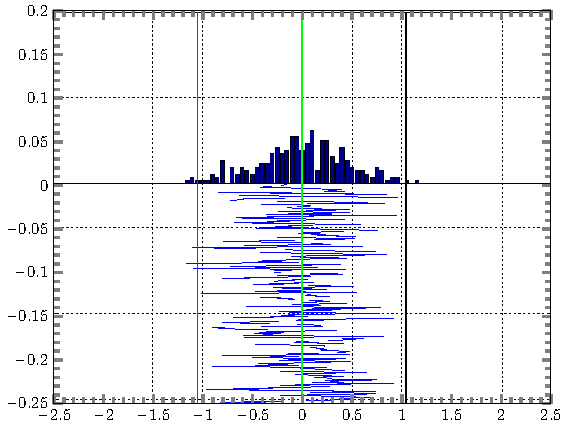
\includegraphics[width=\linewidth]{fig/gist_n4_b98.pdf}
    \vspace{-1em}
    \caption{$\beta =0.98$}
\end{minipage}
\end{figure}

\paragraph{Серия при $N=32$.} \hphantom{asasfsd}
\begin{figure}[H]
\begin{minipage}{0.3\linewidth}
    \centering
    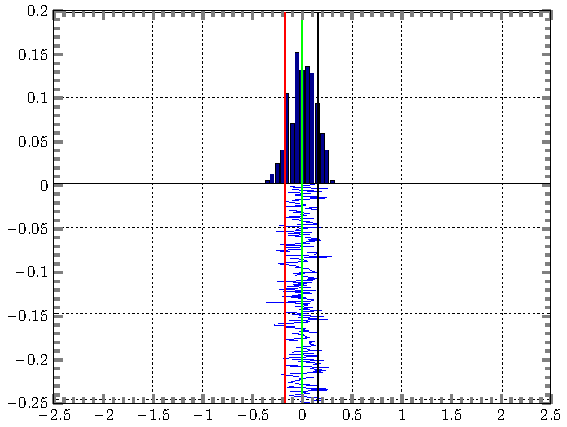
\includegraphics[width=\linewidth]{fig/gist_n32_b80.pdf}
    \vspace{-1em}
    \caption{$\beta =0.8$}
\end{minipage}
\begin{minipage}{0.3\linewidth}
    \centering
    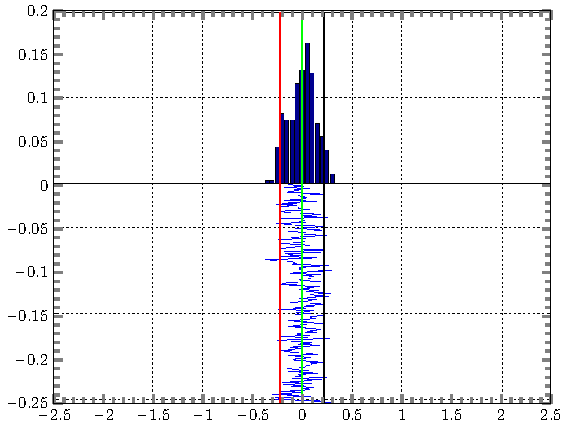
\includegraphics[width=\linewidth]{fig/gist_n32_b95.pdf}
    \vspace{-1em}
    \caption{$\beta =0.95$}
\end{minipage}
\begin{minipage}{0.3\linewidth}
    \centering
    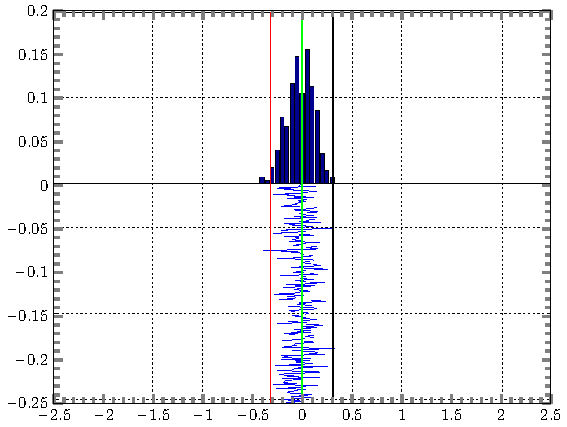
\includegraphics[width=\linewidth]{fig/gist_n32_b98.pdf}
    \vspace{-1em}
    \caption{$\beta =0.98$}
\end{minipage}
\end{figure}

По результатам серии измерений получена зависимость доверительного интервала $I$ от $\beta$ для разных значений $N$:
 \begin{figure}[H]
    \centering
    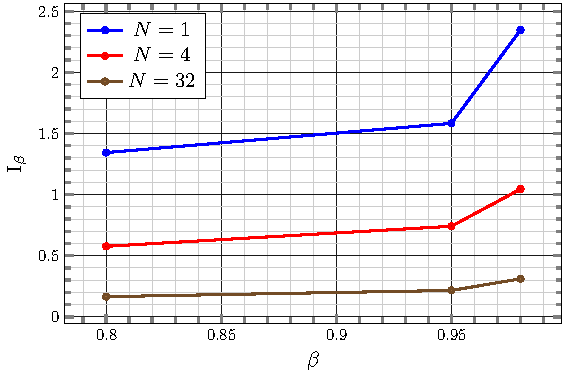
\includegraphics[width=0.8\linewidth]{fig/I_from_beta}
    \caption{График зависимости доверительного интервала $I$ от $\beta$}
\end{figure}
Из графика видно, что доверительный интервал растет с ростом $\beta$ и уменьшается при увеличении окна усреднения ($N\uparrow$).

\addcontentsline{toc}{section}{Заключение}
\section*{Заключение}

В настоящей работе была изучена тема оценка параметров случайных процессов на примере оценки их средних значений. 

С помощью предоставленного кафедрой статистической радиофизики программного обеспечения, позволяющего генерировать и изучать  дискретный гауссов шум с заданными характеристиками, получен ряд качественных выводов о поведении сигнала и спектра при изменении различных параметров: объема ансамбля реализаций, ширины окна усреднения, времени дискретизации усреднения, доверительной вероятности, времени корреляции.

Основные качественные результаты -- вывод о обратной зависимости времени корреляции и ширины спектра сигнала, о прямой зависимости ширины доверительного интервала и доверительной вероятности. 
\end{document}
